

\textit{Con la segmentación realizada en el ejercicio 1 de la señal} \texttt{hh2.wav}\emph{, encuentre los coeficientes
de Fourier de un período del segmento de señal correspondiente a un fono [a]. Repetir el cálculo
para varios períodos de la vocal.}\\

	A continuación se presenta el gráfico del fono [a] seleccionado, que corresponde a la última [a] de la palabra \emph{ahuyentar}. En ella también se presentan los periodos seleccionados para el cálculo de coeficientes.

	\begin{figure}
		\centering
		\scalebox{0.6}{% GNUPLOT: LaTeX picture with Postscript
\begingroup
  \makeatletter
  \providecommand\color[2][]{%
    \GenericError{(gnuplot) \space\space\space\@spaces}{%
      Package color not loaded in conjunction with
      terminal option `colourtext'%
    }{See the gnuplot documentation for explanation.%
    }{Either use 'blacktext' in gnuplot or load the package
      color.sty in LaTeX.}%
    \renewcommand\color[2][]{}%
  }%
  \providecommand\includegraphics[2][]{%
    \GenericError{(gnuplot) \space\space\space\@spaces}{%
      Package graphicx or graphics not loaded%
    }{See the gnuplot documentation for explanation.%
    }{The gnuplot epslatex terminal needs graphicx.sty or graphics.sty.}%
    \renewcommand\includegraphics[2][]{}%
  }%
  \providecommand\rotatebox[2]{#2}%
  \@ifundefined{ifGPcolor}{%
    \newif\ifGPcolor
    \GPcolorfalse
  }{}%
  \@ifundefined{ifGPblacktext}{%
    \newif\ifGPblacktext
    \GPblacktexttrue
  }{}%
  % define a \g@addto@macro without @ in the name:
  \let\gplgaddtomacro\g@addto@macro
  % define empty templates for all commands taking text:
  \gdef\gplbacktext{}%
  \gdef\gplfronttext{}%
  \makeatother
  \ifGPblacktext
    % no textcolor at all
    \def\colorrgb#1{}%
    \def\colorgray#1{}%
  \else
    % gray or color?
    \ifGPcolor
      \def\colorrgb#1{\color[rgb]{#1}}%
      \def\colorgray#1{\color[gray]{#1}}%
      \expandafter\def\csname LTw\endcsname{\color{white}}%
      \expandafter\def\csname LTb\endcsname{\color{black}}%
      \expandafter\def\csname LTa\endcsname{\color{black}}%
      \expandafter\def\csname LT0\endcsname{\color[rgb]{1,0,0}}%
      \expandafter\def\csname LT1\endcsname{\color[rgb]{0,1,0}}%
      \expandafter\def\csname LT2\endcsname{\color[rgb]{0,0,1}}%
      \expandafter\def\csname LT3\endcsname{\color[rgb]{1,0,1}}%
      \expandafter\def\csname LT4\endcsname{\color[rgb]{0,1,1}}%
      \expandafter\def\csname LT5\endcsname{\color[rgb]{1,1,0}}%
      \expandafter\def\csname LT6\endcsname{\color[rgb]{0,0,0}}%
      \expandafter\def\csname LT7\endcsname{\color[rgb]{1,0.3,0}}%
      \expandafter\def\csname LT8\endcsname{\color[rgb]{0.5,0.5,0.5}}%
    \else
      % gray
      \def\colorrgb#1{\color{black}}%
      \def\colorgray#1{\color[gray]{#1}}%
      \expandafter\def\csname LTw\endcsname{\color{white}}%
      \expandafter\def\csname LTb\endcsname{\color{black}}%
      \expandafter\def\csname LTa\endcsname{\color{black}}%
      \expandafter\def\csname LT0\endcsname{\color{black}}%
      \expandafter\def\csname LT1\endcsname{\color{black}}%
      \expandafter\def\csname LT2\endcsname{\color{black}}%
      \expandafter\def\csname LT3\endcsname{\color{black}}%
      \expandafter\def\csname LT4\endcsname{\color{black}}%
      \expandafter\def\csname LT5\endcsname{\color{black}}%
      \expandafter\def\csname LT6\endcsname{\color{black}}%
      \expandafter\def\csname LT7\endcsname{\color{black}}%
      \expandafter\def\csname LT8\endcsname{\color{black}}%
    \fi
  \fi
  \setlength{\unitlength}{0.0500bp}%
  \begin{picture}(11520.00,8640.00)%
    \gplgaddtomacro\gplbacktext{%
      \colorrgb{0.00,0.00,0.00}%
      \put(660,400){\makebox(0,0)[r]{\strut{}-0.8}}%
      \colorrgb{0.00,0.00,0.00}%
      \put(660,1355){\makebox(0,0)[r]{\strut{}-0.6}}%
      \colorrgb{0.00,0.00,0.00}%
      \put(660,2310){\makebox(0,0)[r]{\strut{}-0.4}}%
      \colorrgb{0.00,0.00,0.00}%
      \put(660,3265){\makebox(0,0)[r]{\strut{}-0.2}}%
      \colorrgb{0.00,0.00,0.00}%
      \put(660,4220){\makebox(0,0)[r]{\strut{}0}}%
      \colorrgb{0.00,0.00,0.00}%
      \put(660,5174){\makebox(0,0)[r]{\strut{}0.2}}%
      \colorrgb{0.00,0.00,0.00}%
      \put(660,6129){\makebox(0,0)[r]{\strut{}0.4}}%
      \colorrgb{0.00,0.00,0.00}%
      \put(660,7084){\makebox(0,0)[r]{\strut{}0.6}}%
      \colorrgb{0.00,0.00,0.00}%
      \put(660,8039){\makebox(0,0)[r]{\strut{}0.8}}%
      \colorrgb{0.00,0.00,0.00}%
      \put(976,200){\makebox(0,0){\strut{}2.8}}%
      \colorrgb{0.00,0.00,0.00}%
      \put(2281,200){\makebox(0,0){\strut{}2.82}}%
      \colorrgb{0.00,0.00,0.00}%
      \put(3587,200){\makebox(0,0){\strut{}2.84}}%
      \colorrgb{0.00,0.00,0.00}%
      \put(4892,200){\makebox(0,0){\strut{}2.86}}%
      \colorrgb{0.00,0.00,0.00}%
      \put(6198,200){\makebox(0,0){\strut{}2.88}}%
      \colorrgb{0.00,0.00,0.00}%
      \put(7504,200){\makebox(0,0){\strut{}2.9}}%
      \colorrgb{0.00,0.00,0.00}%
      \put(8809,200){\makebox(0,0){\strut{}2.92}}%
      \colorrgb{0.00,0.00,0.00}%
      \put(10115,200){\makebox(0,0){\strut{}2.94}}%
      \csname LTb\endcsname%
      \put(5969,8339){\makebox(0,0){\strut{}Gráfico del fono "a" (ahuyentar) con los periodos utilizados}}%
    }%
    \gplgaddtomacro\gplfronttext{%
      \colorrgb{0.00,0.00,0.00}%
      \put(2763,1563){\makebox(0,0)[r]{\strut{}Fono "a"}}%
      \colorrgb{0.00,0.00,0.00}%
      \put(2763,1363){\makebox(0,0)[r]{\strut{}Periodo 1}}%
      \colorrgb{0.00,0.00,0.00}%
      \put(2763,1163){\makebox(0,0)[r]{\strut{}Periodo 2}}%
      \colorrgb{0.00,0.00,0.00}%
      \put(2763,963){\makebox(0,0)[r]{\strut{}Periodo 3}}%
      \colorrgb{0.00,0.00,0.00}%
      \put(2763,763){\makebox(0,0)[r]{\strut{}Periodo 4}}%
      \colorrgb{0.00,0.00,0.00}%
      \put(2763,563){\makebox(0,0)[r]{\strut{}Periodo 5}}%
    }%
    \gplbacktext
    \put(0,0){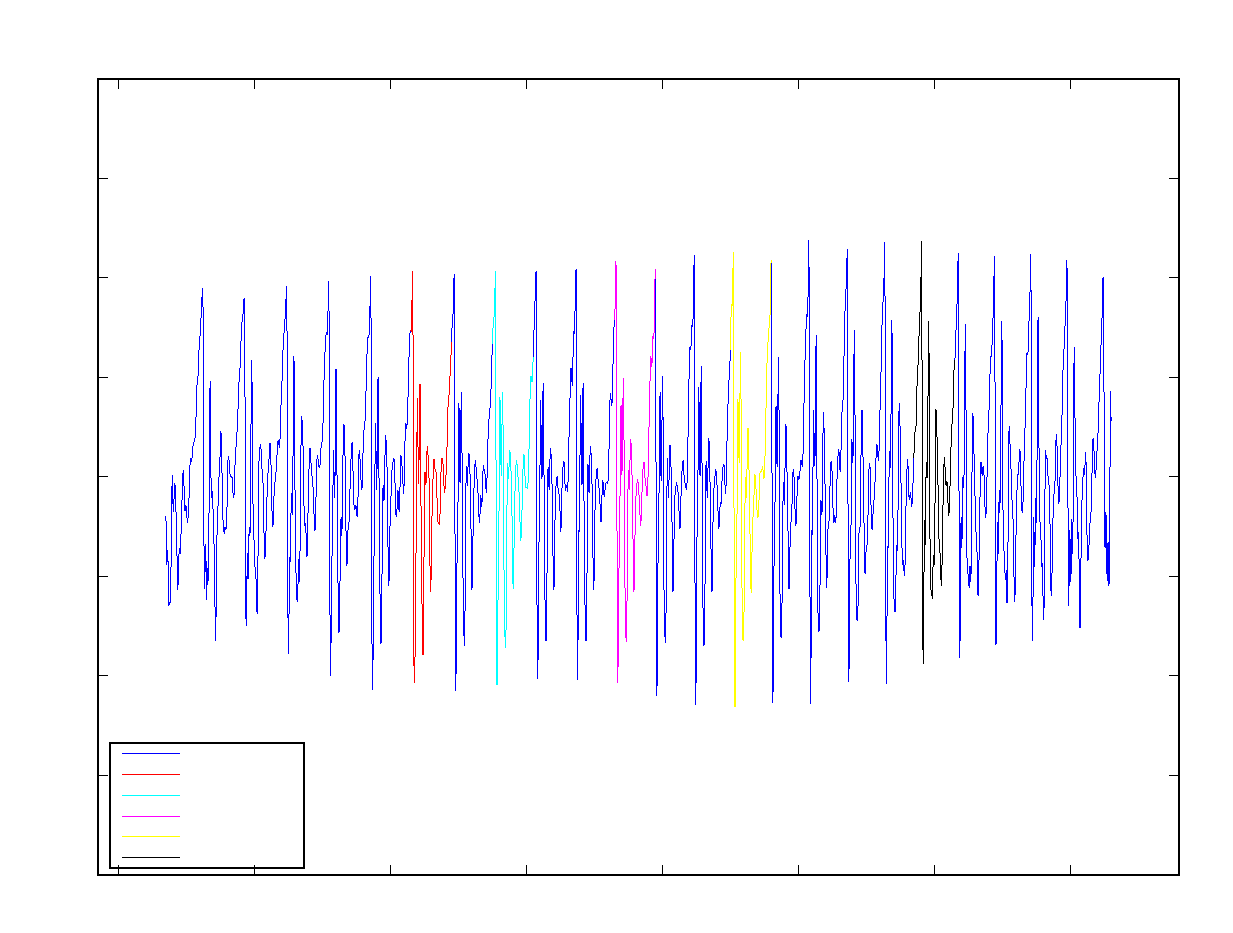
\includegraphics{./graf_fono_a}}%
    \gplfronttext
  \end{picture}%
\endgroup
}
	\end{figure}

	Con los periodos seleccionados previamente, se obtuvieron los coeficientes de Fourier, representados en el siguiente gráfico

	
	\begin{figure}
		\centering
		\scalebox{0.6}{% GNUPLOT: LaTeX picture with Postscript
\begingroup
  \makeatletter
  \providecommand\color[2][]{%
    \GenericError{(gnuplot) \space\space\space\@spaces}{%
      Package color not loaded in conjunction with
      terminal option `colourtext'%
    }{See the gnuplot documentation for explanation.%
    }{Either use 'blacktext' in gnuplot or load the package
      color.sty in LaTeX.}%
    \renewcommand\color[2][]{}%
  }%
  \providecommand\includegraphics[2][]{%
    \GenericError{(gnuplot) \space\space\space\@spaces}{%
      Package graphicx or graphics not loaded%
    }{See the gnuplot documentation for explanation.%
    }{The gnuplot epslatex terminal needs graphicx.sty or graphics.sty.}%
    \renewcommand\includegraphics[2][]{}%
  }%
  \providecommand\rotatebox[2]{#2}%
  \@ifundefined{ifGPcolor}{%
    \newif\ifGPcolor
    \GPcolorfalse
  }{}%
  \@ifundefined{ifGPblacktext}{%
    \newif\ifGPblacktext
    \GPblacktexttrue
  }{}%
  % define a \g@addto@macro without @ in the name:
  \let\gplgaddtomacro\g@addto@macro
  % define empty templates for all commands taking text:
  \gdef\gplbacktext{}%
  \gdef\gplfronttext{}%
  \makeatother
  \ifGPblacktext
    % no textcolor at all
    \def\colorrgb#1{}%
    \def\colorgray#1{}%
  \else
    % gray or color?
    \ifGPcolor
      \def\colorrgb#1{\color[rgb]{#1}}%
      \def\colorgray#1{\color[gray]{#1}}%
      \expandafter\def\csname LTw\endcsname{\color{white}}%
      \expandafter\def\csname LTb\endcsname{\color{black}}%
      \expandafter\def\csname LTa\endcsname{\color{black}}%
      \expandafter\def\csname LT0\endcsname{\color[rgb]{1,0,0}}%
      \expandafter\def\csname LT1\endcsname{\color[rgb]{0,1,0}}%
      \expandafter\def\csname LT2\endcsname{\color[rgb]{0,0,1}}%
      \expandafter\def\csname LT3\endcsname{\color[rgb]{1,0,1}}%
      \expandafter\def\csname LT4\endcsname{\color[rgb]{0,1,1}}%
      \expandafter\def\csname LT5\endcsname{\color[rgb]{1,1,0}}%
      \expandafter\def\csname LT6\endcsname{\color[rgb]{0,0,0}}%
      \expandafter\def\csname LT7\endcsname{\color[rgb]{1,0.3,0}}%
      \expandafter\def\csname LT8\endcsname{\color[rgb]{0.5,0.5,0.5}}%
    \else
      % gray
      \def\colorrgb#1{\color{black}}%
      \def\colorgray#1{\color[gray]{#1}}%
      \expandafter\def\csname LTw\endcsname{\color{white}}%
      \expandafter\def\csname LTb\endcsname{\color{black}}%
      \expandafter\def\csname LTa\endcsname{\color{black}}%
      \expandafter\def\csname LT0\endcsname{\color{black}}%
      \expandafter\def\csname LT1\endcsname{\color{black}}%
      \expandafter\def\csname LT2\endcsname{\color{black}}%
      \expandafter\def\csname LT3\endcsname{\color{black}}%
      \expandafter\def\csname LT4\endcsname{\color{black}}%
      \expandafter\def\csname LT5\endcsname{\color{black}}%
      \expandafter\def\csname LT6\endcsname{\color{black}}%
      \expandafter\def\csname LT7\endcsname{\color{black}}%
      \expandafter\def\csname LT8\endcsname{\color{black}}%
    \fi
  \fi
  \setlength{\unitlength}{0.0500bp}%
  \begin{picture}(11520.00,8640.00)%
    \gplgaddtomacro\gplbacktext{%
      \colorrgb{0.00,0.00,0.00}%
      \put(500,640){\makebox(0,0)[r]{\strut{}0}}%
      \colorrgb{0.00,0.00,0.00}%
      \put(500,1565){\makebox(0,0)[r]{\strut{}1}}%
      \colorrgb{0.00,0.00,0.00}%
      \put(500,2490){\makebox(0,0)[r]{\strut{}2}}%
      \colorrgb{0.00,0.00,0.00}%
      \put(500,3415){\makebox(0,0)[r]{\strut{}3}}%
      \colorrgb{0.00,0.00,0.00}%
      \put(500,4340){\makebox(0,0)[r]{\strut{}4}}%
      \colorrgb{0.00,0.00,0.00}%
      \put(500,5264){\makebox(0,0)[r]{\strut{}5}}%
      \colorrgb{0.00,0.00,0.00}%
      \put(500,6189){\makebox(0,0)[r]{\strut{}6}}%
      \colorrgb{0.00,0.00,0.00}%
      \put(500,7114){\makebox(0,0)[r]{\strut{}7}}%
      \colorrgb{0.00,0.00,0.00}%
      \put(500,8039){\makebox(0,0)[r]{\strut{}8}}%
      \colorrgb{0.00,0.00,0.00}%
      \put(620,440){\makebox(0,0){\strut{}0}}%
      \colorrgb{0.00,0.00,0.00}%
      \put(1937,440){\makebox(0,0){\strut{}500}}%
      \colorrgb{0.00,0.00,0.00}%
      \put(3255,440){\makebox(0,0){\strut{}1000}}%
      \colorrgb{0.00,0.00,0.00}%
      \put(4572,440){\makebox(0,0){\strut{}1500}}%
      \colorrgb{0.00,0.00,0.00}%
      \put(5890,440){\makebox(0,0){\strut{}2000}}%
      \colorrgb{0.00,0.00,0.00}%
      \put(7207,440){\makebox(0,0){\strut{}2500}}%
      \colorrgb{0.00,0.00,0.00}%
      \put(8524,440){\makebox(0,0){\strut{}3000}}%
      \colorrgb{0.00,0.00,0.00}%
      \put(9842,440){\makebox(0,0){\strut{}3500}}%
      \colorrgb{0.00,0.00,0.00}%
      \put(11159,440){\makebox(0,0){\strut{}4000}}%
      \colorrgb{0.00,0.00,0.00}%
      \put(160,4339){\rotatebox{90}{\makebox(0,0){\strut{}|X|}}}%
      \colorrgb{0.00,0.00,0.00}%
      \put(5889,140){\makebox(0,0){\strut{}Frecuencia [Hz]}}%
      \csname LTb\endcsname%
      \put(5889,8339){\makebox(0,0){\strut{}Respuesta en frecuencia de los periodos seleccionados del fono "a" (ahuyentar)}}%
    }%
    \gplgaddtomacro\gplfronttext{%
      \colorrgb{0.00,0.00,0.00}%
      \put(11039,7876){\makebox(0,0)[r]{\strut{}Periodo 1}}%
      \colorrgb{0.00,0.00,0.00}%
      \put(11039,7676){\makebox(0,0)[r]{\strut{}Periodo 2}}%
      \colorrgb{0.00,0.00,0.00}%
      \put(11039,7476){\makebox(0,0)[r]{\strut{}Periodo 3}}%
      \colorrgb{0.00,0.00,0.00}%
      \put(11039,7276){\makebox(0,0)[r]{\strut{}Periodo 4}}%
      \colorrgb{0.00,0.00,0.00}%
      \put(11039,7076){\makebox(0,0)[r]{\strut{}Periodo 5}}%
    }%
    \gplbacktext
    \put(0,0){\includegraphics{./graf_coef}}%
    \gplfronttext
  \end{picture}%
\endgroup
}
	\end{figure}
